\chapter{Wyniki eksperymentalne}
\thispagestyle{chapterBeginStyle}
\label{rozdzial3}

W tym rozdziale pokazano wyniki testów dla prezentowanego programu oraz porównano go z innymi istniejącymi rozwiązaniami. 
Wszystkie eksperymenty zostały wykonane na serwerze Politechniki Wrocławskiej - \textit{OTRYT}. Serwer jest wyposażony w 4 procesory 
\textit{Intel(R) Xeon(R) CPU E7- 4850  @ 2.00GHz} posiadające po 10 rdzeni każdy oraz w 256 GB pamięci RAM. Serwer działa pod systemem 
\textit{Linux Debian} w wersji \textit{9.11}.

Dane testowe pochodzą częściowo z książki dr. Michalewicza(zadania $7 \times 7$ oraz $10 \times 10$)\cite{ALG-GEN-BOOK}, a częściowo 
zostały wygenerowane. Sposób generowania danych zaczerpnięto z publikacji \cite{GEN-TEST-DATA}. Dla wektorów popytu i podaży ustalano 
całkowity popyt/podaż, a następnie wypełniano je losowymi liczbami, zachowując przy tym warunek całkowitego popytu i podaży. 
Macierz kosztu generowano w taki sposób, że na początku ustalano dolne i górne ograniczenie wartości pojedynczego przewozu, a następnie 
macierz wypełniano losowymi liczbami z ustalonego zakresu. W przypadku jednej z funkcji kosztu, potrzebna była również macierz, która 
określa koszt stały, jaki ponosimy niezależnie od ilości towaru przewożonego między punktami. Macierz ta jest generowana w taki sam 
sposób, jak macierz kosztu. Charakterystyka poszczególnych zadań znajduje się w tabeli \ref{specyfika-zadan}.

\begin{table}[H]
    \begin{center}
        \begin{tabular}{c|c|c|c|c}
            Rozmiar & Popyt & Podaż & Zakres dla macierzy kosztu & Zakres dla macierzy kosztów stałych \\ 
            \hline
            $15 \times 15$ & $15000$ & $15000$ & $[3, 8]$ & $[50, 200]$ \\
            $30 \times 30$ & $3000$ & $3000$ & $[5, 15]$ & $[100, 400]$ \\
            $20 \times 70$ & $30000$ & $30000$ & $[3, 8]$ & $[200, 800]$ \\
            $30 \times 60$ & $25000$ & $25000$ & $[5, 15]$ & $[50, 100]$ \\
            $100 \times 100$ & $45000$ & $45000$ & $[3, 8]$ & $[100, 400]$ \\
        \end{tabular}
    \end{center}
    \caption{Charakterystyka wygenerowanych zadań.}
    \label{specyfika-zadan}
\end{table}


Funkcje kosztu użyte w testach w większości pochodzą z książki \cite{ALG-GEN-BOOK}. Przedstawiono je w tabeli \ref{funkcje-kosztu}. Dodatkowo 
użyto funkcji kosztu, która w przypadku przewozu towaru dodaje do kosztów liniowych koszt stały (Funkcja G w tabeli \ref{funkcje-kosztu}).

W eksperymentach porównano przedstawiany algorytm z wybranymi solverami wspieranymi przez system \textbf{GAMS}. Dostęp do solverów był możliwy poprzez serwis 
\textbf{NEOS Server} \cite{NEOS-1,NEOS-2,NEOS-3}, który pozwala na używanie kilkudziesięciu różnych solverów do optymalizacji problemów różnej kategorii. Do wybranych 
solverów należą:

\begin{itemize}
    \item LINDOGlobal
    \item CPLEX
    \item MINOS
    \item SNOPT
    \item scip
\end{itemize}

\newpage

\begin{table}[H]
    \begin{center}
        \begin{tabular}{ccl}
            Funkcja liniowa: & $f(x_{i,j})=$ & $c_{i,j} x_{i,j}$ \\
            \hline
            Funkcja A: & $f(x_{i,j})=$ & $c_{i,j}(\text{arctg}(1000 (x {i,j} - S))/\pi + 0.5 +$ \\
            & & $\text{arctg}(1000 (x {i,j} - 2 S))/\pi + 0.5 +$ \\
            & & $\text{arctg}(1000 (x {i,j} - 3 S))/\pi + 0.5 +$ \\
            & & $\text{arctg}(1000 (x {i,j} - 4 S))/\pi + 0.5 +$ \\
            & & $\text{arctg}(1000 (x {i,j} - 5 S))/\pi + 0.5)$ \\ 
            \hline
            Funkcja B: & $f(x_{i,j})=$ & $c_{i,j}[(x_{i,j}/5) (\text{arctg}(1000 x_{i,j})/\pi + 0.5) +$ \\
            & & $(1 - x_{i,j}/5) (\text{arctg}(1000(x_{i,j} - 5))/\pi + 0.5) +$ \\
            & & $(x_{i,j}/5 - 2) (\text{arctg}(1000(x_{i,j} - 10))/\pi + 0.5)]$ \\
            \hline
            Funkcja C: & $f(x_{i,j})=$ & $c_{i,j} x_{i,j}^2$ \\
            \hline
            Funkcja D: & $f(x_{i,j})=$ & $c_{i,j} \sqrt{x_{i,j}}$ \\
            \hline
            Funkcja E: & $f(x_{i,j})=$ & $c_{i,j}[(1 + (x_{i,j} - 10)^2)^{-1} +$ \\
            & & $(1 + (x_{i,j} - 11.25)^2)^{-1} +$ \\
            & & $(1 + (x_{i,j} - 8.75)^2)^{-1}]$ \\
            \hline
            Funkcja F: & $f(x_{i,j})=$ & $c_{i,j} x_{i,j} (\sin(5 \pi x_{i,j}/20) + 1)$ \\
            \hline
            Funkcja G: & $f(x_{i,j})=$ & $c_{i,j} x_{i,j} + c'_{i,j} y_{i,j}$ \\
        \end{tabular}
    \end{center}
    \caption{Funkcje kosztu}
    \label{funkcje-kosztu}
\end{table}

Z uwagi na to że serwis NEOS narzuca limit czasowy na wykonywanie pojedynczego zadania, przedstawione rozwiązania są najlepszym wynikiem znalezionym 
przez solver w czasie nie większym niż 8 godzin.

W następnych sekcjach zaprezentowano wyniki dla dwóch przedstawionych w poprzednim rozdziale modeli równoległości. Na początku zaprezentowano wyniki 
dla modelu klasycznego, który operuje na jednej populacji. Następnie z wynikami solverów zestawiono wyniki modelu wyspowego, w którym 
populacja jest dzielona na populacje częściowe. Na końcu porównano ze sobą oba modele.

Aby dostosować parametry dla testowanego systemu, na początku przeprowadzono serię testów dla różnych zadań i na podstawie tych wyników ustawiono 
odpowiednio parametry programu:

\begin{itemize}
    \item Rozmiar populacji: $100$(model klasyczny), $400$(model wyspowy)
    \item Prawdopodobieństwo krzyżowania: $0.5$
    \item Prawdopodobieństwo mutacji: $0.1$
    \item Wielkość mutacji: $0.05$
    \item Ułamek najlepszych osobników przepisywanych do nowej generacji: $0.2$
    \item Ilość niezależnych generacji dla populacji częściowej(model wyspowy): $50$
\end{itemize}

Maksymalną ilość iteracji algorytmu ustalono na $30000$.

\section{Model klasyczny algorytmu ewolucyjnego}

Wyniki przeprowazdone dla modelu klasycznego znajdują się w tabelach \ref{wyniki-0} oraz \ref{wyniki-1}. Tabela \ref{wyniki-0} zawiera porównanie 
modelu klasycznego z systemem GENOCOP (wyniki pochodzą z książki\cite{ALG-GEN-BOOK}), który pozwala optymalizować wszelkiego rodzaju zadania z ograniczeniami liniowymi i nieliniową funkcją celu. 
Widzimy tutaj, że nasz algorytm wypada lepiej niż system GENOCOP w większości testów. Udało się to osiągnąć dzięki zastosowaniu w algorytmie wiedzy o zadaniu
i dostosowaniu do niego reprezentacji rozwiązania oraz operatorów. Niestety nie udało się uzyskać wyników GENOCOPA dla zadania rozmiaru 
$10 \times 10$.

\newpage

\begin{table}[H]
    \begin{center}
        \resizebox{\textwidth}{!}{%
        \begin{tabular}{c|c|c|c|c|c|c}
            Rozmiar & Funkcja & \multicolumn{3}{c|}{Model klasyczny} & GENOCOP & LindoGlobal \\ \cline{3-5}
            zadania & celu & min & śr  & max &  & \\ 
            \hline
            \hline
            $7 \times 7$ & Liniowa & $1132.03$ & $1203.98$ & $1265.20$ & $---$ & $1132.0$ \\
            $7 \times 7$ & A & $0.0$ & $13.62$ & $67.0$ & $24.15$ & $4.26$ \\
            $7 \times 7$ & B & $180.65$ & $193.31$ & $224.07$ & $205.60$ & $183.59$ \\
            $7 \times 7$ & C & $2535.29$ & $2535.29$ & $2535.29$ & $2571.04$ & $2535.29$ \\
            $7 \times 7$ & D & $480.16$ & $565.57$ & $1046.45$ & $480.16$ & $480.16$ \\
            $7 \times 7$ & E & $204.71$ & $206.64$ & $221.52$ & $204.82$ & $204.84$ \\
            $7 \times 7$ & F & $67.31$ & $196.48$ & $351.38$ & $119.61$ & $70.25$ \\
            $7 \times 7$ & G & $1813.99$ & $1856.83$ & $1916.12$ & $---$ & $1796.0$ \\
            \hline
            $10 \times 10$ & Liniowa & $1179.0$ & $1188.96$ & $1213.24$ & $---$ & $1179.0$ \\
            $10 \times 10$ & A & $192.0$ & $200.2$ & $212.0$ & $---$ & $174.07$ \\
            $10 \times 10$ & B & $147.15$ & $154.19$ & $166.82$ & $---$ & $146.99$ \\
            $10 \times 10$ & C & $4401.65$ & $4401.65$ & $4401.65$ & $---$ & $4401.65$ \\
            $10 \times 10$ & D & $388.41$ & $409.36$ & $459.0$ & $---$ & $388.91$ \\
            $10 \times 10$ & E & $71.66$ & $72.99$ & $75.48$ & $---$ & $71.66$ \\
            $10 \times 10$ & F & $118.57$ & $215.90$ & $300.21$ & $---$ & $153.49$ \\
            $10 \times 10$ & G & $2010.50$ & $2075.15$ & $2194.69$ & $---$ & $1987.14$ \\
        \end{tabular}
        }
    \end{center}
    \caption{Wyniki dla zadań rozmiaru $7 \times 7$ i $10 \times 10$.}
    \label{wyniki-0}
\end{table}

Tabela \ref{wyniki-1} przedstawia wyniki dla pozostałych zadań wygenerowanych w sposób opisany na początku tego rozdziału. Porównano tutaj model klasyczny 
algorytmu ewolucyjnego z solverami MINOS oraz LINDOGlobal. O ile w przypadku MINOSa nie wiemy czy zwrócona wartość jest optimum globalnym, o tyle 
solver LINDOGlobal informuje o tym czy znalezione rozwiązanie to optimum lokalne czy globalne. Dodatkowo w przypadku optimum lokalnego, podaje on 
informację o najlepszym obliczonym dolnym ograniczeniu minimalizowanej funkcji. 

W przypadku jeśli LINDO zwrócił jedynie optimum lokalne przy wyniku znajduje się litera \textit{L}, w przypadku jeśli znaleziono optimum globalne, 
wynik jest oznaczony literą \textit{G}. W kolumnie \textit{luka} znaje się błąd względny między wartością otrzymaną a optimum globalnym, 
a więc $luka = \frac{|OPT - \tilde{C}|}{|OPT|} 100 \%$. W przypadku jeśli optimum globalne nie zostało znalezione, wiemy że w pesymistycznym 
przypadku znajduje się ono nie dalej niż ograniczenie dolne, tzn. $LB \le OPT$, gdzie $LB$ - ograniczenie dolne wyniku, oraz $OPT$ - optimum 
lokalne znalezione przez solver. W takim przypadku luka jest obliczana jako błąd względny między znalezionym rozwiązaniem, a dolnym ograniczeniem 
funkcji, czyli $luka = \frac{|LB - \tilde{C}|}{|LB|}$. 

Warto zwrócić uwagę na fakt, że podane dolne ograniczenie może być złej jakości, przez co błąd względny może wydawać się bardzo duży. Sytuacja 
taka miała miejsce w przypadku funkcji B oraz F, gdzie ograniczenie dolne dla wszystkich zestawów zadań testowych było równe $0$, czyli najmniejszemu 
możliwemu wynikowi w każdym zadaniu transportowym (z założenia wiemy, że koszt nie może być ujemny).

\newpage

\begin{table}[H]
    \begin{center}
        \resizebox{\textwidth}{!}{%
        \begin{tabular}{c|c||c|c|c|c||c||c|c||c|c}
            Rozmiar         & Funkcja      & \multicolumn{4}{c||}{Model klasyczny}               & MINOS         & \multicolumn{2}{c||}{LindoGlobal}& \multicolumn{2}{c}{CPLEX} \\ \cline{3-6} \cline{8-9} \cline{10-11}
            zadania         & celu         & min & śr  & max & luka                             &               & wynik & luka                    & wynik & luka \\
            \hline  
            \hline  
            $15 \times 15$ & Liniowa       & $54533.80$ & $55062.96$ & $55419.21$ & $1.24$      & $53862.32$    & $53862.32$ G & $0.00$           & $53862.32$ G & $0.00$ \\
            $15 \times 15$ & A             & $621.52$ & $627.98$ & $679.35$ & $40.42$           & $743.05$      & $470.50$ L & $21.27$            & $-$ & $-$ \\
            $15 \times 15$ & B             & $10607.71$ & $10657.78$ & $10933.70$ & $-$(*)      & $10581.32$    & $10454.80$ L & $-$(*)           & $-$ & $-$ \\
            $15 \times 15$ & C             & $5225274.22$ & $5225274.24$ & $5225274.30$ & $0.00$& $5225274.19$  & $5225274.19$ G & $0.00$         & $-$ & $-$ \\
            $15 \times 15$ & D             & $2187.99$ & $2211.11$ & $2273.07$ & $-$(*)         & $3229.68$     & $2314.41$ L & $-$(*)            & $-$ & $-$ \\
            $15 \times 15$ & E             & $1.20$ & $1.20$ & $1.20$ & $-$(*)                  & $33.13$       & $1.90$ L & $-$(*)               & $-$ & $-$ \\
            $15 \times 15$ & F             & $179.61$ & $180.16$ & $185.35$ & $-$(*)            & $11852.89$    & $59.23$ L & $-$(*)              & $-$ & $-$ \\
            $15 \times 15$ & G             & $62185.11$ & $62438.42$ & $63610.24$ & $9.65$      & $57366.75$    & $58546.32$ L & $2.74$           & $56985.03$ G & $0.00$ \\
            \hline  
            $30 \times 30$ & Liniowa       & $17365.25$ & $17479.06$ & $17795.71$ & $4.69$      & $16586.20$    & $16586.20$ G & $0.00$           & $16586.20$ G & $0.00$ \\
            $30 \times 30$ & A             & $1763.86$ & $1795.62$ & $1846.44$ & $27.60$        & $2260.7914$   & $2040.23$ L & $36.27$           & $-$ & $-$ \\
            $30 \times 30$ & B             & $2309.83$ & $2323.66$ & $2370.13$ & $-$(*)         & $2699.25$     & $2696.38$ L & $-$(*)            & $-$ & $-$ \\
            $30 \times 30$ & C             & $104650.12$ & $104650.40$ & $104651.73$ & $0.00$   & $104650.12$   & $104650.12$ G & $0.00$          & $-$ & $-$ \\
            $30 \times 30$ & D             & $2872.53$ & $2986.45$ & $3084.81$ & $-$(*)         & $3805.08$     & $2770.29$ L & $-$(*)            & $-$ & $-$ \\
            $30 \times 30$ & E             & $249.70$ & $249.84$ & $256.32$ & $61.33$           & $262.08$      & $285.34$ L & $66.14$            & $-$ & $-$ \\
            $30 \times 30$ & F             & $737.98$ & $823.82$ & $1063.14$ & $-$(*)           & $4630.83$     & $384.87$ L & $-$(*)             & $-$ & $-$ \\
            $30 \times 30$ & G             & $23533.16$ & $24813.93$ & $26622.49$ & $27.43$     & $19912.58$    & $20117.31$ L & $3.25$           & $19482.41$ G & $0.00$ \\
            \hline  
            $20 \times 70$ & Liniowa       & $102681.39$ & $102980.75$ & $103318.46$ & $4.57$   & $98476.50$    & $98476.50$ G & $0.00$           & $98476.50$ G & $0.00$ \\
            $20 \times 70$ & A             & $1926.42$ & $1997.94$ & $2099.43$ & $50.56$        & $2437.58$     & $1473.70$ L & $32.98$           & $-$ & $-$ \\
            $20 \times 70$ & B             & $19294.37$ & $19777.36$ & $20164.15$ & $-$(*)      & $19164.16$    & $18524.19$ L & $-$(*)           & $-$ & $-$ \\
            $20 \times 70$ & C             & $3356726.47$ & $3356779.29$ & $3356994.88$ & $0.00$& $3356719.33$  & $3356719.33$ G & $0.00$         & $-$ & $-$ \\
            $20 \times 70$ & D             & $6703.65$ & $6747.31$ & $6823.62$ & $-$(*)         & $8947.35$     & $6245.85$ L & $-$(*)            & $-$ & $-$ \\
            $20 \times 70$ & E             & $111.69$ & $113.03$ & $114.37$ & $-$(*)            & $221.51$      & $139.55$ L & $-$(*)             & $-$ & $-$ \\
            $20 \times 70$ & F             & $1594.30$ & $1644.51$ & $1697.70$ & $-$(*)         & $40503.51$    & $575.38$ L & $-$(*)             & $-$ & $-$ \\
            $20 \times 70$ & G             & $169931.77$ & $172399.15$ & $179244.49$ & $30.61$  & $135150.04$   & $134327.33$ L & $1.81$          & $131938.45$ G & $0.00$ \\
            \hline  
            $30 \times 60$ & Liniowa       & $145468.29$ & $146323.93$ & $146948.53$ & $7.67$   & $135028.71$   & $135028.71$ G & $0.00$          & $135028.71$ G & $0.00$ \\
            $30 \times 60$ & A             & $3532.37$ & $3544.40$ & $3631.18$ & $53.30$        & $4310.14$     & $2336.59$ L & $29.17$           & $-$ & $-$ \\
            $30 \times 60$ & B             & $26033.88$ & $26962.21$ & $27024.11$ & $-$(*)      & $26082.37$    & $26775.34$ L & $-$(*)           & $-$ & $-$ \\
            $30 \times 60$ & C             & $3283244.35$ & $3283249.33$ & $3283363.39$ & $0.00$& $3282784.56$  & $3282784.56$ G & $0.00$         & $-$ & $-$ \\
            $30 \times 60$ & D             & $11090.32$ & $11172.53$ & $11275.56$ & $-$(*)      & $13799.71$    & $Time out$ & $-$(*)             & $-$ & $-$ \\
            $30 \times 60$ & E             & $351.38$ & $351.57$ & $351.74$ & $-$(*)            & $526.34$      & $438.39$ L & $-$(*)             & $-$ & $-$ \\
            $30 \times 60$ & F             & $2981.06$ & $3498.70$ & $4404.37$ & $-$(*)         & $73724.43$    & $2390.12$ L & $-$(*)            & $-$ & $-$ \\
            $30 \times 60$ & G             & $176947.28$ & $180834.11$ & $187061.33$ & $27.54$  & $143907.24$   & $145316.08$ L & $2.51$          & $141761.66$ G & $0.00$ \\
            \hline  
            $100 \times 100$ & Liniowa     & $152120.75$ & $157299.10$ & $163931.16$ & $-$      & $138605.09$   & $Err$ & $-$                     & $138605.09$ G & $0.00$ \\
            $100 \times 100$ & A           & $4162.49$ & $4176.67$ & $4180.39$ & $-$            & $Err$         & $Err$ & $-$                     & $-$ & $-$ \\
            $100 \times 100$ & B           & $27175.45$ & $27320.57$ & $27993.08$ & $-$         & $Err$         & $Err$ & $-$                     & $-$ & $-$ \\
            $100 \times 100$ & C           & $1079937.33$ & $1080471.39$ & $1081882.67$ & $-$   & $Err$         & $Err$ & $-$                     & $-$ & $-$ \\
            $100 \times 100$ & D           & $12308.57$ & $12414.59$ & $12991.94$ & $-$         & $Err$         & $Err$ & $-$                     & $-$ & $-$ \\
            $100 \times 100$ & E           & $1531.03$ & $1531.32$ & $1532.51$ & $-$            & $Err$         & $Err$ & $-$                     & $-$ & $-$ \\
            $100 \times 100$ & F           & $---$ & $7405.57$ & $---$ &                        & $Err$         & $Err$ & $-$                     & $-$ & $-$ \\
            $100 \times 100$ & G           & $232139.70$ & $235821.75$ & $239278.53$ & $37.20$  & $175472.60$   & $Err$ & $-$                     & $171871.92$ G & $0.00$ \\
        \end{tabular}
        } 
    \end{center}
    \caption{Wyniki. (*) oznacza, że znalezione ograniczenie dolne dla problemu było słabej jakości, tzn. że było równe, lub bardzo bliskie $0$. 
        Wynik \textit{Timeout} oznacza, że solver nie znalazł rozwiązania w czasie 8 godzin. 
        Wynik \textit{Err} oznacza, że model był za duży dla solvera.}
    \label{wyniki-1}
\end{table}


Jak możemy zauważyć na prezentowanym porównaniu (tabela \ref{wyniki-1}) model klasyczny wypada lepiej niż solver MINOS w niemalże każdym teście. Jedyny 
wyjątek stanowi przypadek liniowej funkcji kosztu, gdzie MINOS zawsze znajdował optimum globalne. W przypadku funkcji B MINOS wypadał nieznacznie 
lepiej niż średni wynik dla modelu klasycznego, jednak była to z reguły różnica pomijalna (poniżej $1\%$). Z kolei dla funkcji D oraz F model 
klasyczny był znacznie lepszy niż MINOS, który w niektórych przypadkach zwrócił nawet kilkukrotnie gorszy wynik (funkcja F). Pozostałe wyniki były raczej 
zbliżone. Dla funkcji nieliniowych A-G i macierzy $100 \times 100$ MINOS nie zwrócił żadnego wyniku, ze względu na ograniczone zasoby pamięci oferowane 
przez serwis NEOS. 

Dla solvera LINDOGlobal, w wielu przypadkach wynikiem obliczeń było jedynie optimum lokalne (funkcje A,B,D,E,F). W tych przypadkach możemy 
porównywać odległości od dolnego ograniczenia wyniku wskazanego przez LINDOGlobal. Jest ono jednak w wielu przypadkach bardzo nieprecyzyjne. 
Mimo wszystko dla większości testów model klasyczny dawał wyniki zbliżone do wynkiów solvera. Przypadki łatwe, w których zostało znalezione optimum 
globalne były rozwiązywane przez model klasyczny z akceptowalnym błędem rzędu kilku procent.

Możemy zauważyć, że w przypadku liniowej funkcji kosztu model klasyczny radzi sobie gorzej niż pozostałe programy, jest to jednak problem bardzo 
łatwy i znamy dużo lepsze algorytmy, któwe są w stanie w krótkim czasie znaleźć dla niego optimum globalne. W tego typu prostych zadaniach stosowanie 
algorytmów metaheurystycznych, do których zalicza się opisywany algorytm ewolucyjny raczej mija się z celem. Stosunkowo słabe wyniki w tym przypadku 
są wynikiem tego, że otrzymywane osobniki nie są wystarczająco zróżnicowane. Z kolei dla dużo trudniejszych, nieliniowych 
funkcji celu, model klasyczny radzi sobie znacznie lepiej. Przede wszystkim prezentuje się dużo lepiej niż pozostałe solvery w porównaniu czasu 
potrzebnego na znalezienie rozwiązania. Dla algorytmu ewolucyjnego nawet problem rozmiaru $100 \times 100$ nie był żadną trudnością i 
był rozwiązywany w czasie kilkudziesięciu sekund. Pokazuje to główną zaletę algorytmów ewolucyjnych, jaką jest czas znajdowania rozwiązania.

Z uwagi na to, że w wielu przypadkach LINDO nie znalazł optimum globalnego, a ograniczenie dolne było niezadowalającej jakości, zdecydowano się 
porównać wyniki algorytmu ewolucyjnego z wynikami innych solverów, które również są w stanie optymalizować nieliniową funkcję celu 
przy liniowych ograniczeniach. Porównanie to znajduje się w tabeli \ref{wyniki-2}. Dla zwiększenia czytelności w tabeli pokazano jedynie średni wynik 
zwracany przez algorytm ewolucyjny. W kolumnach oznaczonych jako \% pokazano błąd względny pomiędzy najlepszym wynikiem dla konkretnego testu oraz 
wynikiem solvera. Takie porównanie daje lepszy obraz tego, jak prezentowany algorytm ewolucyjny wypada na tle innych istniejących rozwiązań.

\begin{table}[H]
    \begin{center}
        \resizebox{\textwidth}{!}{%
        \begin{tabular}{c|c||c|c||c|c||c|c||c|c||c|c}
            Rozmiar         & Funkcja    & \multicolumn{2}{c||}{Model klasyczny}  & \multicolumn{2}{c||}{MINOS} & \multicolumn{2}{c||}{scip} & \multicolumn{2}{c||}{SNOPT}& \multicolumn{2}{c}{LindoGlobal} \\ \cline{3-4} \cline{5-6} \cline{7-8} \cline{9-10} \cline{11-12}
            zadania         & celu       & śr. wynik & \%                        & wynik & \%                 & wynik & \%                & wynik & \%                & wynik & \% \\
            \hline
            \hline
            $15 \times 15$ & Liniowa     & $55062.96$ & $2.2$                    & $53862.32$ & \textbf{0.0}         & $53862.32$ & \textbf{0.0}        & $53862.32$ & \textbf{0.00}       & $53862.32$ & \textbf{0.0} \\
            $15 \times 15$ & A           & $627.98$ & $33.4$                     & $743.05$ & $57.9$          & $696.75$ & $48.1$         & $743.05$ & $57.9$         & $470.50$ & \textbf{0.0} \\
            $15 \times 15$ & B           & $10657.78$ & $1.9$                    & $10581.32$ & $1.2$         & $10630.82$ & $1.7$        & $10510.23$ & $0.5$        & $10454.80$ & \textbf{0.0} \\
            $15 \times 15$ & C           & $5225274.24$ & \textbf{0.0}                  & $5225274.19$ & \textbf{0.0}       & $5225274.19$ & \textbf{0.0}      & $5225274.19$ & \textbf{0.0}      & $5225274.19$ & \textbf{0.0} \\
            $15 \times 15$ & D           & $2211.11$ & \textbf{0.0}                     & $3229.68$ & $46.1$         & $2867.07$ & $29.7$        & $3229.68$ & $46.1$        & $2314.41$ & $4.67$ \\
            $15 \times 15$ & E           & $1.20$ & \textbf{0.0}                        & $33.13$ & $2660.8$         & $20.41$ & $1600.8$        & $33.50$ & $2691.7$        & $1.90$ & $58.3$ \\
            $15 \times 15$ & F           & $180.16$ & $204.2$                    & $11852.89$ & $19911.6$     & $2646.60$ & $4368.3$      & $10150.31$ & $17037.1$    & $59.23$ & \textbf{0.0} \\
            $15 \times 15$ & G           & $62438.42$ & $8.9$                    & $57366.75$ & \textbf{0.0}         & $57327.80$ & \textbf{0.0}        & $57366.75$ & \textbf{0.0}        & $58546.32$ & $2.1$ \\
            \hline
            $30 \times 30$ & Liniowa     & $17479.06$ & $5.4$                    & $16586.20$ & \textbf{0.0}         & $16586.20$ & \textbf{0.0}        & $16586.20$ & \textbf{0.0}        & $16586.20$ & \textbf{0.0} \\
            $30 \times 30$ & A           & $1795.62$ & \textbf{0.0}                     & $2260.7914$ & $25.9$       & $1888.26$ & $5.15$        & $2295.27$ & $27.8$        & $2040.23$ & $13.6$ \\
            $30 \times 30$ & B           & $2323.66$ & \textbf{0.0}                     & $2699.25$ & $16.2$         & $2664.35$ & $14.7$        & $2547.94$ & $9.7$         & $2696.38$ & $16.0$ \\
            $30 \times 30$ & C           & $104650.40$ & \textbf{0.0}                   & $104650.12$ & \textbf{0.0}        & $104650.12$ & \textbf{0.0}       & $144947.97$ & $38.5$      & $104650.12$ & \textbf{0.0} \\
            $30 \times 30$ & D           & $2986.45$ & $7.8$                     & $3805.08$ & $37.3$         & $3410.94$ & $23.1$        & $3805.08$ & $37.3$        & $2770.29$ & \textbf{0.0} \\
            $30 \times 30$ & E           & $249.84$ & \textbf{0.0}                      & $262.08$ & $4.9$           & $309.33$ & $23.8$         & $262.08$ & $4.9$          & $285.34$ & $14.2$ \\
            $30 \times 30$ & F           & $823.82$ & $114.0$                    & $4630.83$ & $1103.2$       & $957.32$ & $148.7$        & $4171.94$ & $984.0$       & $384.87$ & \textbf{0.0} \\
            $30 \times 30$ & G           & $24813.93$ & $24.6$                   & $19912.58$ & \textbf{0.0}         & $19981.01$ & $0.4$        & $19912.58$ & \textbf{0.0}        & $20117.31$ & $1.0$ \\
            \hline
            $20 \times 70$ & Liniowa     & $102980.75$ & $4.6$                   & $98476.50$ & \textbf{0.0}         & $98476.50$ & \textbf{0.0}        & $98476.50$ & \textbf{0.0}        & $98476.50$ & \textbf{0.0} \\
            $20 \times 70$ & A           & $1997.94$ & $35.5$                    & $2437.58$ & $65.4$         & $1781.99$ & $20.9$        & $2437.58$ & $65.4$        & $1473.70$ & \textbf{0.0} \\
            $20 \times 70$ & B           & $19777.36$ & $7.26$                   & $19164.16$ & $3.9$         & $18763.24$ & $1.8$        & $18438.52$ & \textbf{0.0}        & $18524.19$ & $0.5$ \\
            $20 \times 70$ & C           & $3356779.29$ & \textbf{0.0}                  & $3356719.33$ & \textbf{0.0}       & $3356719.33$ & \textbf{0.0}      & $7808433.26$ & $132.6$    & $3356719.33$ & \textbf{0.0} \\
            $20 \times 70$ & D           & $6747.31$ & $11.6$                    & $8947.35$ & $47.9$         & $6047.94$ & \textbf{0.0}         & $8947.35$ & $47.9$        & $6245.85$ & $3.27$ \\
            $20 \times 70$ & E           & $113.03$ & \textbf{0.0}                      & $221.51$ & $96.0$          & $176.21$ & $56.0$         & $221.51$ & $96.0$         & $139.55$ & $23.5$ \\
            $20 \times 70$ & F           & $1644.51$ & $186.0$                   & $40503.51$ & $6939.4$      & $7462.94$ & $1197.0$      & $40939.03$ & $7015.1$     & $575.38$ & \textbf{0.0} \\
            $20 \times 70$ & G           & $172399.15$ & $28.3$                  & $135150.04$ & $0.6$        & $135150.0$ & $0.6$        & $135150.0$ & $0.6$        & $134327.33$ & \textbf{0.0} \\
            \hline
            $30 \times 60$ & Liniowa     & $146323.93$ & $8.3$                   & $135028.71$ & \textbf{0.0}        & $135028.71$ & \textbf{0.0}       & $135028.71$ & \textbf{0.0}       & $135028.71$ & \textbf{0.0} \\
            $30 \times 60$ & A           & $3544.40$ & $51.7$                    & $4310.14$ & $84.5$         & $3767.46$ & $61.2$        & $4310.14$ & $84.5$        & $2336.59$ & \textbf{0.0} \\
            $30 \times 60$ & B           & $26962.21$ & $7.3$                    & $26082.37$ & $3.8$         & $26355.05$ & $4.9$        & $25126.84$ & \textbf{0.0}        & $26775.34$ & $6.6$ \\
            $30 \times 60$ & C           & $3283249.33$ & \textbf{0.0}                  & $3282784.56$ & \textbf{0.0}       & $3282784.56$ & \textbf{0.0}      & $9640058.72$ & $193.7$    & $3282784.56$ & \textbf{0.0} \\
            $30 \times 60$ & D           & $11172.53$ & $0.8$                    & $13799.71$ & $24.5$        & $11081.48$ & \textbf{0.0}        & $13799.71$ & $24.5$       & $Time out$ & $-$ \\
            $30 \times 60$ & E           & $351.57$ & \textbf{0.0}                      & $526.34$ & $49.7$          & $1158.46$ & $230.0$       & $526.34$ & $49.7$         & $438.39$ & $24.7$ \\
            $30 \times 60$ & F           & $3498.70$ & $46.4$                    & $73724.43$ & $2984.5$      & $6935.45$ & $190.2$       & $68411.66$ & $2762.3$     & $2390.12$ & \textbf{0.0} \\
            $30 \times 60$ & G           & $180834.11$ & $25.6$                  & $143907.24$ & \textbf{0.0}        & $143953.62$ & $0.1$       & $143907.24$ & \textbf{0.0}        & $145316.08$ & $0.9$ \\
            \hline
            $100 \times 100$ & Liniowa   & $157299.10$ & $13.5$                  & $138605.09$ & \textbf{0.0}        & $138605.09$ & \textbf{0.0}       & $138605.09$ & \textbf{0.0}       & $Err$ & $-$ \\
            $100 \times 100$ & A         & $4176.67$ & \textbf{0.0}                     & $Err$ & $-$                & $4657.38$ & $11.5$        & $25858.31$ & $519.1$      & $Err$ & $-$ \\
            $100 \times 100$ & B         & $27320.57$ & \textbf{0.0}                    & $Err$ & $-$                & $35556.19$ & $30.1$       & $35556.19$ & $30.1$       & $Err$ & $-$ \\
            $100 \times 100$ & C         & $1080471.39$ & $1.3$                  & $Err$ & $-$                & $1066457.36$ & \textbf{0.0}      & $15080858.45$ & $1314.1$  & $Err$ & $-$ \\
            $100 \times 100$ & D         & $12414.59$ & \textbf{0.0}                    & $Err$ & $-$                & $13910.55$ & $12.1$       & $15844.99$ & $27.6$       & $Err$ & $-$ \\
            $100 \times 100$ & E         & $1531.32$ & \textbf{0.0}                     & $Err$ & $-$                & $1741.40$ & $13.7$        & $1657.65$ & $8.2$         & $Err$ & $-$ \\
            $100 \times 100$ & F         & $7405.57$ & \textbf{0.0}                     & $Err$ & $-$                & $10064.85$ & $36.0$       & $31191.89$ & $321.2$      & $Err$ & $-$ \\
            $100 \times 100$ & G         & $235821.75$ & $34.3$                  & $175472.60$ & \textbf{0.0}        & $175517.69$ & \textbf{0.0}       & $175472.60$ & \textbf{0.0}       & $Err$ & $-$ \\
        \end{tabular}
        }
    \end{center}
    \caption{Porównanie modelu klasycznego algorytmu ewolucyjnego i innych dostępnych solverów.}
    \label{wyniki-2}
\end{table}

Jakość rozwiązań zwracanych przez algorytm ewolucyjny jest zadowalająca. Łatwo zauważyć, że radzi on sobie najgorzej w zadaniach z liniową funkcją celu 
oraz z funkcją G, która dodaje do kosztu transportu koszt stały. Powodem tego jest to, że w tych przypadkach wiemy, że rozwiązanie optymalne jest 
wierzchołkiem przestrzeni dopuszczalnych rozwiązań (przy zadaniu z funkcją liniową\cite{ALG-GEN-BOOK}), lub przeważają w nim elementy zerowe (funkcja G). 
W takich przypadkach prezentowany algorytm wypada gorzej, ponieważ używany operator krzyżowania sprawia, że elementów zerowych w rozwiązaniu 
jest bardzo mało. Operatorem, który wprowadza elementy zerowe do rozwiązania jest operator mutacji i nawet jeśli znaczne zwiększenie prawdopodobieństwa 
mutacji może poprawić wyniki dla tych przypadków, to algorytm działa wtedy dużo bardziej jak przeszukiwanie losowe. W obu przypadkach, w których 
algorytm genetyczny wypadał dużo gorzej, pozostałe solvery radziły sobie bardzo dobrze, w szczególności CPLEX, który w każdym z tych przypadków zwrócił 
optimum globalne. 

Warto zwrócić uwagę na fakt, że warianty zadania z funkcją liniową oraz z dodatkowymi kosztami stałymi są dość łatwe i 
standardowe metody optymalizacji bez problemu sobie z nimi radzą. W takiej sytuacji metody przeszukiwania przestrzeni rozwiązań w postaci algorytmów 
metaheurystycznych nie będą tak dobre jak dokładne metody optymalizacji, więc ich stosowanie jest zbędne. Metaheurystyki powinny być stosowane 
przede wszystkim tam, gdzie klasyczne metody nie dają nam zadowalających rezultatów.

W pozostałych zadaniach algorytm wypada bardzo dobrze. Konkurować z nim może tylko solver LINDO, który jednak potrzebuje znacznie więcej czasu, 
aby wyliczyć optymalne rozwiązanie. Dodatkowo posiada on dość mały limit zmiennych, co nie pozwoliło na obliczenie zadania rozmiaru $100 \times 100$. 
Pozostałe solvery radziły sobie w tych przypadkach gorzej niż algorytm ewolucyjny.

\newpage

\section{Model wyspowy algorytmu ewolucyjnego}

W tabeli \ref{wyniki-3} zaprezentowano wyniki dla wyspowego modelu algorytmu ewolucyjnego.

\begin{table}[H]
    \begin{center}
        \resizebox{\textwidth}{!}{%
        \begin{tabular}{c|c||c|c||c|c||c|c||c|c||c|c}
            Rozmiar         & Funkcja    & \multicolumn{2}{c||}{Model wyspowy}   & \multicolumn{2}{c||}{MINOS} & \multicolumn{2}{c||}{scip} & \multicolumn{2}{c||}{SNOPT}& \multicolumn{2}{c}{LindoGlobal} \\ \cline{3-4} \cline{5-6} \cline{7-8} \cline{9-10} \cline{11-12}
            zadania         & celu       & śr. wynik & \%                        & wynik & \%                 & wynik & \%                & wynik & \%                & wynik & \% \\
            \hline
            \hline
            $15 \times 15$ & Liniowa     & $55624.17$ & $3.27$                   & $53862.32$ & \textbf{0.0}         & $53862.32$ & \textbf{0.0}        & $53862.32$ & \textbf{0.00}       & $53862.32$ & \textbf{0.0} \\
            $15 \times 15$ & A           & $632.36$ & $34.4$                     & $743.05$ & $57.9$          & $696.75$ & $48.1$         & $743.05$ & $57.9$         & $470.50$ & \textbf{0.0} \\
            $15 \times 15$ & B           & $10588.37$ & $1.2$                    & $10581.32$ & $1.2$         & $10630.82$ & $1.7$        & $10510.23$ & $0.5$        & $10454.80$ & \textbf{0.0} \\
            $15 \times 15$ & C           & $5229421.80$ & \textbf{0.0}                  & $5225274.19$ & \textbf{0.0}       & $5225274.19$ & \textbf{0.0}      & $5225274.19$ & \textbf{0.0}      & $5225274.19$ & \textbf{0.0} \\
            $15 \times 15$ & D           & $2320.71$ & $0.2$                     & $3229.68$ & $46.1$         & $2867.07$ & $29.7$        & $3229.68$ & $46.1$        & $2314.41$ & $4.67$ \\
            $15 \times 15$ & E           & $1.29$ & \textbf{0.0}                        & $33.13$ & $2468.2$         & $20.41$ & $1482.2$        & $33.50$ & $2496.9$        & $1.90$ & $47.3$ \\
            $15 \times 15$ & F           & $162.26$ & $173.9$                    & $11852.89$ & $19911.6$     & $2646.60$ & $4368.3$      & $10150.31$ & $17037.1$    & $59.23$ & \textbf{0.0} \\
            $15 \times 15$ & G           & $60949.33$ & $6.2$                    & $57366.75$ & \textbf{0.0}         & $57327.80$ & \textbf{0.0}        & $57366.75$ & \textbf{0.0}        & $58546.32$ & $2.1$ \\
            \hline
            $30 \times 30$ & Liniowa     & $17298.37$ & $4.3$                    & $16586.20$ & \textbf{0.0}         & $16586.20$ & \textbf{0.0}        & $16586.20$ & \textbf{0.0}        & $16586.20$ & \textbf{0.0} \\
            $30 \times 30$ & A           & $1416.35$ & \textbf{0.0}                     & $2260.79$ & $59.6$       & $1888.26$ & $33.3$        & $2295.27$ & $62.1$        & $2040.23$ & $44.0$ \\
            $30 \times 30$ & B           & $2271.24$ & \textbf{0.0}                     & $2699.25$ & $18.8$         & $2664.35$ & $17.3$        & $2547.94$ & $12.2$         & $2696.38$ & $18.7$ \\
            $30 \times 30$ & C           & $107383.37$ & $2.6$                   & $104650.12$ & \textbf{0.0}        & $104650.12$ & \textbf{0.0}       & $144947.97$ & $38.5$      & $104650.12$ & \textbf{0.0} \\
            $30 \times 30$ & D           & $2566.87$ & \textbf{0.0}                     & $3805.08$ & $48.2$         & $3410.94$ & $32.9$        & $3805.08$ & $48.2$        & $2770.29$ & $7.9$ \\
            $30 \times 30$ & E           & $245.82$ & \textbf{0.0}                      & $262.08$ & $6.6$           & $309.33$ & $25.8$         & $262.08$ & $6.6$          & $285.34$ & $16.1$ \\
            $30 \times 30$ & F           & $604.63$ & $57.1$                     & $4630.83$ & $1103.2$       & $957.32$ & $148.7$        & $4171.94$ & $984.0$       & $384.87$ & \textbf{0.0} \\
            $30 \times 30$ & G           & $23820.57$ & $19.6$                   & $19912.58$ & \textbf{0.0}         & $19981.01$ & $0.4$        & $19912.58$ & \textbf{0.0}        & $20117.31$ & $1.0$ \\
            \hline
            $20 \times 70$ & Liniowa     & $102803.27$ & $4.4$                   & $98476.50$ & \textbf{0.0}         & $98476.50$ & \textbf{0.0}        & $98476.50$ & \textbf{0.0}        & $98476.50$ & \textbf{0.0} \\
            $20 \times 70$ & A           & $1706.41$ & $15.8$                    & $2437.58$ & $65.4$         & $1781.99$ & $20.9$        & $2437.58$ & $65.4$        & $1473.70$ & \textbf{0.0} \\
            $20 \times 70$ & B           & $20138.18$ & $9.2$                    & $19164.16$ & $3.9$         & $18763.24$ & $1.8$        & $18438.52$ & \textbf{0.0}        & $18524.19$ & $0.5$ \\
            $20 \times 70$ & C           & $3363917.33$ & $0.2$                  & $3356719.33$ & \textbf{0.0}       & $3356719.33$ & \textbf{0.0}      & $7808433.26$ & $132.6$    & $3356719.33$ & \textbf{0.0} \\
            $20 \times 70$ & D           & $5780.16$ & \textbf{0.0}                    & $8947.35$ & $54.8$         & $6047.94$ & $4.6$         & $8947.35$ & $54.8$        & $6245.85$ & $8.1$ \\
            $20 \times 70$ & E           & $165.30$ & $18.5$                      & $221.51$ & $58.7$          & $176.21$ & $26.3$         & $221.51$ & $58.7$         & $139.55$ & \textbf{0.0} \\
            $20 \times 70$ & F           & $1961.35$ & $240.9$                   & $40503.51$ & $6939.4$      & $7462.94$ & $1197.0$      & $40939.03$ & $7015.1$     & $575.38$ & \textbf{0.0} \\
            $20 \times 70$ & G           & $165520.67$ & $23.2$                  & $135150.04$ & $0.6$        & $135150.0$ & $0.6$        & $135150.0$ & $0.6$        & $134327.33$ & \textbf{0.0} \\
            \hline
            $30 \times 60$ & Liniowa     & $145532.36$ & $7.8$                   & $135028.71$ & \textbf{0.0}        & $135028.71$ & \textbf{0.0}       & $135028.71$ & \textbf{0.0}       & $135028.71$ & \textbf{0.0} \\
            $30 \times 60$ & A           & $2991.78$ & $28.0$                    & $4310.14$ & $84.5$         & $3767.46$ & $61.2$        & $4310.14$ & $84.5$        & $2336.59$ & \textbf{0.0} \\
            $30 \times 60$ & B           & $28553.81$ & $13.6$                    & $26082.37$ & $3.8$         & $26355.05$ & $4.9$        & $25126.84$ & \textbf{0.0}        & $26775.34$ & $6.6$ \\
            $30 \times 60$ & C           & $3299166.19$ & $0.5$                  & $3282784.56$ & \textbf{0.0}       & $3282784.56$ & \textbf{0.0}      & $9640058.72$ & $193.7$    & $3282784.56$ & \textbf{0.0} \\
            $30 \times 60$ & D           & $9461.37$ & \textbf{0.0}                    & $13799.71$ & $45.9$        & $11081.48$ & $17.1$        & $13799.71$ & $45.9$       & $Time out$ & $-$ \\
            $30 \times 60$ & E           & $341.81$ & \textbf{0.0}                      & $526.34$ & $54.0$          & $1158.46$ & $238.9$       & $526.34$ & $54.0$         & $438.39$ & $28.3$ \\
            $30 \times 60$ & F           & $3560.92$ & $49.0$                    & $73724.43$ & $2984.5$      & $6935.45$ & $190.2$       & $68411.66$ & $2762.3$     & $2390.12$ & \textbf{0.0} \\
            $30 \times 60$ & G           & $165912.53$ & $15.3$                  & $143907.24$ & \textbf{0.0}        & $143953.62$ & $0.1$       & $143907.24$ & \textbf{0.0}        & $145316.08$ & $0.9$ \\
            \hline
            $100 \times 100$ & Liniowa   & $160326.25$ & $15.7$                  & $138605.09$ & \textbf{0.0}        & $138605.09$ & \textbf{0.0}       & $138605.09$ & \textbf{0.0}       & $Err$ & $-$ \\
            $100 \times 100$ & A         & $3641.13$ & \textbf{0.0}                     & $Err$ & $-$                & $4657.38$ & $27.9$        & $25858.31$ & $610.2$      & $Err$ & $-$ \\
            $100 \times 100$ & B         & $27241.74$ & \textbf{0.0}                    & $Err$ & $-$                & $35556.19$ & $30.5$       & $35556.19$ & $30.5$       & $Err$ & $-$ \\
            $100 \times 100$ & C         & $1121317.16$ & $5.1$                  & $Err$ & $-$                & $1066457.36$ & \textbf{0.0}      & $15080858.45$ & $1314.1$  & $Err$ & $-$ \\
            $100 \times 100$ & D         & $11626.03$ & \textbf{0.0}                    & $Err$ & $-$                & $13910.55$ & $19.7$       & $15844.99$ & $36.3$       & $Err$ & $-$ \\
            $100 \times 100$ & E         & $1597.67$ & \textbf{0.0}                     & $Err$ & $-$                & $1741.40$ & $9.0$        & $1657.65$ & $3.8$         & $Err$ & $-$ \\
            $100 \times 100$ & F         & $6792.93$ & \textbf{0.0}                     & $Err$ & $-$                & $10064.85$ & $48.2$       & $31191.89$ & $359.2$      & $Err$ & $-$ \\
            $100 \times 100$ & G         & $235512.39$ & $34.2$                  & $175472.60$ & \textbf{0.0}        & $175517.69$ & \textbf{0.0}       & $175472.60$ & \textbf{0.0}       & $Err$ & $-$ \\
        \end{tabular}
        }
    \end{center}
    \caption{Porównanie modelu wyspowego algorytmu ewolucyjnego i innych dostępnych solverów.}
    \label{wyniki-3}
\end{table}

Widzimy, że prezentuje się on podobnie do modelu klasycznego (tabela \ref{wyniki-4}). W większości testowych przypadków wypada on lepiej lub bardzo 
podobnie do pozostałych solverów. LINDOGlobal znowu wygrywa w przypadku najłatwiejszych z testowanych przypadków. W przypadku modelu rozmiaru 
$100 \times 100$ widzimy znaczącą przewagę algorytmu ewolucyjnego nad dwoma pozostałymi (scip oraz SNOPT), które poradziły sobie z tak dużym 
modelem (w przypadku solvera MINOS ilość pamięci wymagana do rozwiązania zadania przekroczyła limit oferowany przez NEOS).

Podobnie jak w klasycznym modelu najgorzej wypadają zadania z funkcją liniową oraz funkcją z uwzględniającą stały koszt początkowy(G), ze względu 
na poziom trudności tych zadań. 

Modele klasyczny i wyspowy, dały nam zadowalające rezultaty w postaci znajdowanych rozwiązań. W obu przypadkach lepszy okazał się LINDOGlobal, ale tak 
jak zostało wspomniane wcześniej czas jakiego potrzebował on na znalezienie rozwiązania był dużo dłuższy. Pozostałe solvery wypadły już dużo gorzej.

\section{Porównanie modelu klasycznego i wyspowego}

Jak pokazano w poprzednich sekcjach, otrzymywane wyniki są podobnej jakości nie zależnie od użytego modelu zrównoleglenia. Atutem modelu wyspowego 
jest fakt, że każda z populacji jest niezależna i dzięki temu może przeszukiwać inną część przestrzeni rozwiązań\cite{ISLAND-MODEL-PERFORMANCE}, 
co może skutkować lepszą zbieżnością algorytmu i znajdowaniem rozwiązań bliżej optimum globalnego.

% // TABELA

Tabela \ref{wyniki-4} pokazuje porównanie średnich wyników dla obu prezentowanych modeli algorytmu ewolucyjnego. Widzimy, że w znacznej ilości 
przypadków testowych wersja wyspowa radzi sobie lepiej niż wersja klasyczna. Szczególnie widoczne jest to w przypadku testów z funkcją celu G, 
gdzie model wyspowy zawsze znalazł rozwiązanie lepsze niż wersja klasyczna. Warto zauważyć, że w przypadku tej funkcji znamy optimum globalne, 
ponieważ jest ono wyliczane przez solver CPLEX. Jest to wynik tego, że model wyspowy posiada kilka populacji częściowych, które składają się 
z innych osobników. Dzięki temu każda z populacji może przeszukiwać inną część przestrzeni rozwiązań, co ułatwia znalezienie lepszego rozwiązania. 
W wyniku tego, że populacje częściowe są co jakiś czas łączone i mieszane, prawdopodobieństwo zatrzymania się algorytmu w optimum lokalnym 
znacząco spada. 

\newpage

\begin{table}[H]
    \begin{center}
        \begin{tabular}{c|c||c|c||c|c}
            Rozmiar         & Funkcja    & \multicolumn{2}{c||}{Model klasyczny}  & \multicolumn{2}{c}{Model wyspowy} \\ \cline{3-4} \cline{5-6}
            zadania         & celu       & śr. wynik & \%                        & śr. wynik & \%                 \\
            \hline
            \hline
            $15 \times 15$ & Liniowa     & $55062.96$ & \textbf{0.0}             & $55624.17$ & $1.0$ \\
            $15 \times 15$ & A           & $627.98$ & \textbf{0.0}               & $632.36$ & $0.7$ \\
            $15 \times 15$ & B           & $10657.78$ & $0.7$                    & $10588.37$ & \textbf{0.0} \\
            $15 \times 15$ & C           & $5225274.24$ & \textbf{0.0}           & $5229421.80$ & $0.1$ \\
            $15 \times 15$ & D           & $2211.11$ & \textbf{0.0}              & $2320.71$ & $5.0$ \\
            $15 \times 15$ & E           & $1.20$ & \textbf{0.0}                 & $1.29$ & $7.5$ \\
            $15 \times 15$ & F           & $180.16$ & $11.0$                     & $162.26$ & \textbf{0.0} \\
            $15 \times 15$ & G           & $62438.42$ & $2.4$                    & $60949.33$ & \textbf{0.0} \\
            \hline
            $30 \times 30$ & Liniowa     & $17479.06$ & $1.0$                    & $17298.37$ & \textbf{0.0} \\
            $30 \times 30$ & A           & $1795.62$ & $26.8$                    & $1416.35$ & \textbf{0.0} \\
            $30 \times 30$ & B           & $2323.66$ & $2.3$                     & $2271.24$ & \textbf{0.0} \\
            $30 \times 30$ & C           & $104650.40$ & \textbf{0.0}            & $107383.37$ & $2.6$ \\
            $30 \times 30$ & D           & $2986.45$ & $16.3$                    & $2566.87$ & \textbf{0.0} \\
            $30 \times 30$ & E           & $249.84$ & $1.6$                      & $245.82$ & \textbf{0.0} \\
            $30 \times 30$ & F           & $823.82$ & $36.3$                     & $604.63$ & \textbf{0.0} \\
            $30 \times 30$ & G           & $24813.93$ & $4.2$                    & $23820.57$ & \textbf{0.0} \\
            \hline
            $20 \times 70$ & Liniowa     & $102980.75$ & $0.2$                   & $102803.27$ & \textbf{0.0} \\
            $20 \times 70$ & A           & $1997.94$ & $17.0$                    & $1706.41$ & \textbf{0.0} \\
            $20 \times 70$ & B           & $19777.36$ & \textbf{0.0}             & $20138.18$ & $1.8$ \\
            $20 \times 70$ & C           & $3356779.29$ & \textbf{0.0}           & $3363917.33$ & $0.2$ \\
            $20 \times 70$ & D           & $6747.31$ & $16.7$                    & $5780.16$ & \textbf{0.0} \\
            $20 \times 70$ & E           & $113.03$ & \textbf{0.0}               & $165.30$ & $46.2$ \\
            $20 \times 70$ & F           & $1644.51$ & \textbf{0.0}              & $1961.35$ & $19.3$ \\
            $20 \times 70$ & G           & $172399.15$ & $4.2$                   & $165520.67$ & \textbf{0.0} \\
            \hline
            $30 \times 60$ & Liniowa     & $146323.93$ & $0.5$                   & $145532.36$ & \textbf{0.0} \\
            $30 \times 60$ & A           & $3544.40$ & $18.5$                    & $2991.78$ & \textbf{0.0} \\
            $30 \times 60$ & B           & $26962.21$ & \textbf{0.0}             & $28553.81$ & $6.0$ \\
            $30 \times 60$ & C           & $3283249.33$ & \textbf{0.0}           & $3299166.19$ & $0.5$ \\
            $30 \times 60$ & D           & $11172.53$ & $18.1$                   & $9461.37$ & \textbf{0.0} \\
            $30 \times 60$ & E           & $351.57$ & $2.9$                      & $341.81$ & \textbf{0.0} \\
            $30 \times 60$ & F           & $3498.70$ & \textbf{0.0}              & $3560.92$ & $1.8$ \\
            $30 \times 60$ & G           & $180834.11$ & $9.0$                   & $165912.53$ & \textbf{0.0} \\
            \hline
            $100 \times 100$ & Liniowa   & $157299.10$ & \textbf{0.0}            & $160326.25$ & $2.0$ \\
            $100 \times 100$ & A         & $4176.67$ & $14.7$                    & $3641.13$ & \textbf{0.0} \\
            $100 \times 100$ & B         & $27320.57$ & $0.3$                    & $27241.74$ & \textbf{0.0} \\
            $100 \times 100$ & C         & $1080471.39$ & \textbf{0.0}           & $1121317.16$ & $3.7$ \\
            $100 \times 100$ & D         & $12414.59$ & $6.8$                    & $11626.03$ & \textbf{0.0} \\
            $100 \times 100$ & E         & $1531.32$ & $4.3$                     & $1597.67$ & \textbf{0.0} \\
            $100 \times 100$ & F         & $7405.57$ & $9.0$                     & $6792.93$ & \textbf{0.0} \\
            $100 \times 100$ & G         & $235821.75$ & $0.1$                   & $235512.39$ & \textbf{0.0} \\
        \end{tabular}
    \end{center}
    \caption{Porównanie modelu klasycznego i modelu wyspowego algorytmu ewolucyjnego.}
    \label{wyniki-4}
\end{table}

Przyjżyjmy się teraz temu, jaki zysk w postaci skrócenia czasu znalezienia rozwiązania, udało nam się osiągnąć dzięki zastosowanym modelom 
zrównoleglenia. Wykresy \ref{threads_regular_100x100} oraz \ref{threads_island_100x100} pokazują jak wygląda zależność czasu wykonania 10000 iteracji 
algorytmu dla populacji liczącej 400 osobników w przypadku zadania rozmiaru $100 \times 100$. Na wykresie \ref{threads_comparsion_100x100} 
zaprezentowano porównanie obu modeli dla tych samych danych. 

\begin{figure}[H]
    \centering        
    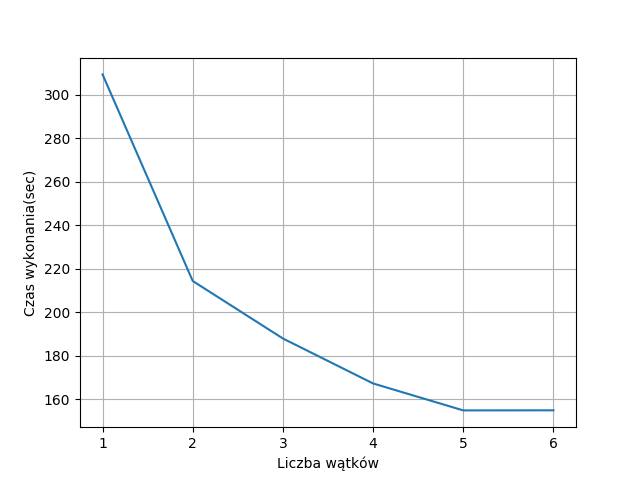
\includegraphics[width=0.6\textwidth]{img/plot_regular_threads_100x100.png}
    \caption{Zależność czasu wykonania programu od ilości używanych wątków dla modelu klasycznego dla zadania rozmiaru $100\times100$.}
    \label{threads_regular_100x100}
\end{figure}

\begin{figure}[H]
    \centering        
    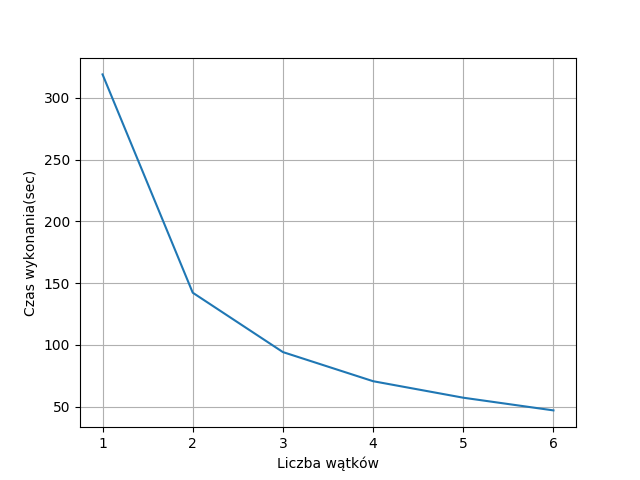
\includegraphics[width=0.6\textwidth]{img/plot_island_threads_100x100.png}
    \caption{Zależność czasu wykonania programu od ilości używanych wątków dla modelu wyspowego dla zadania rozmiaru $100\times100$.}
    \label{threads_island_100x100}
\end{figure}

\begin{figure}[H]
    \centering        
    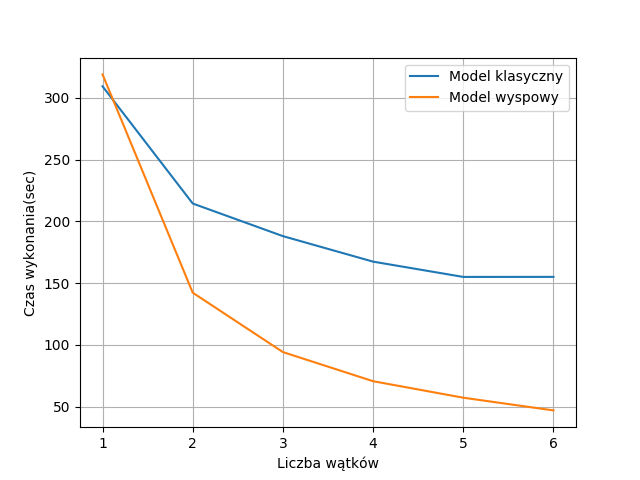
\includegraphics[width=0.6\textwidth]{img/plot_compare_threads_100x100.png}
    \caption{Porównanie modeli klasycznego i wyspowego pod względem zależności czasu wykonania programu od ilości używanych wątków dla zadania 
    rozmiaru $100\times100$.}
    \label{threads_comparsion_100x100}
\end{figure}

Możemy zauważyć, że spadek czasu wykonania jest dużo większy w przypadku modelu wyspowego (wykres \ref{threads_comparsion_100x100}). 
Wynika to z tego, że rozmiar zadania przydzielanego wątkom 
jest dużo większy w modelu wyspowym, niż w modelu klasycznym. Wprowadza on jednak dodatkowy warunek, czyli odpowiednio większą populacje. To znaczy, że 
im więcej wątków angażujemy, tym większa powinna być populacja całkowita, ponieważ jest ona rozdzielana na równe części, na przykład dla populacji 50 
osobników uruchomienie 10 wątków nie miałoby sensu z uwagi na to, że każdy działałby na 5 osobnikach. Skutkowałoby to bardzo szybką zbieżnością algorytmu, 
a co za tym idzie słabej jakości wynikami. Przykład pokazano na wykresie \ref{zla_zbieznosc_watki}. Uruchomiono model wyspowy z całkowitą populacją 40 osobników 
dla 2, 4 i 8 wątków. Wykres przedstawia ewolucje kosztu najlepszego osobnika na przestrzeni 10000 pokoleń.

\begin{figure}[H]
    \centering        
    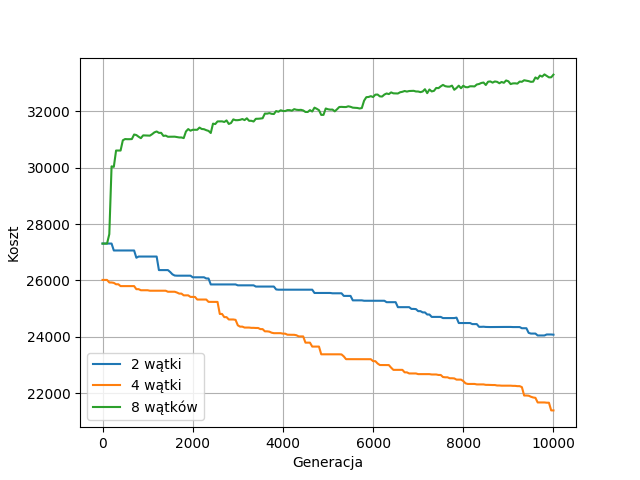
\includegraphics[width=0.6\textwidth]{img/zla_zbieznosc_watki.png}
    \caption{Ewolucja populacji 40 osobników dla 2, 4 i 8 populacji częściowych.}
    \label{zla_zbieznosc_watki}
\end{figure}

Widzimy tutaj, że w przypadku zastosowania 8 populacji częściowych koszt zamiast maleć na przestrzeni pokoleń, rośnie. Pokazuje to, że odpowiednio 
duży rozmiar populacji jest wymagany, aby algorytm ewolucyjny działał poprawnie.

Używanie dużej ilości wątków w przypadku modelu klasycznego ma sens podczas rozwiązywania bardzo dużych zadań. W mniejszych problemach dodatkowy narzut w 
postaci podziału zadań, komunikacji oraz synchronizacji jest większy niż zysk płynący z równoległości, przez co podniesienie ilości używanych wątków ponad 
określoną liczbę skutkuje zwiększeniem czasu potrzebnego na znalezienie rozwiązania. 

W celu lepszego pokazania jak rozmiar zadania wpływa na spadek czasu potrzebnego do zakończenia obliczeń wraz z dodaniem kolejnych wątków, wygenerowano 
dwa dodatkowe zadania rozmiaru $500 \times 500$ oraz $1000 \times 1000$. Następnie zmierzono czas obliczeń używając od 1 do 25 wątków. Dla większej 
przejrzystości przeskalowano wyniki w taki sposób, żeby oś y określała stosunek czasu obliczeń, do czasu potrzebnego przy użyciu 1 wątku. Rezultat 
pokazano na wykresie \ref{threads_comparsion_500x500_1000x1000}

\begin{figure}[H]
    \centering        
    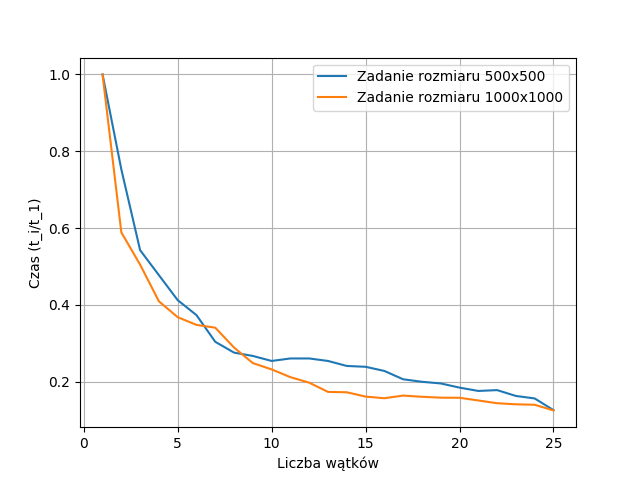
\includegraphics[width=0.6\textwidth]{img/compare_500_1000.png}
    \caption{Porównanie czasu dla zadań rozmiaru $500 \times 500$ i $1000 \times 1000$.}
    \label{threads_comparsion_500x500_1000x1000}
\end{figure}

Widzimy, że w przypadku większego zadania spadek czasu był większy wraz z dokładaniem kolejnych wątków, niż w przypadku mniejszego zadania. Dzieje się 
tak, ponieważ większe zadania przydzielane poszczególnym wątkom wydłużają czas współbieżnego działania aplikacji, jednocześnie nie zmieniając czasu
potrzebnego na synchronizację. Barierą, której nie jesteśmy jednak w stanie przeskoczyć 
są fragmenty kodu, które nie pozwalają się zrównoleglić oraz dodatkowy czas, którego potrzebuje garbage collector Julii na zarządzanie dostępną pamięcią. 
Wynikiem tego jest wypłaszczenie wykresu w miarę wzrostu wartości na osi x.

Porównując oba modele możemy dojść do wniosku, że algorytm wykorzystujący model wyspowy jest lepszy niż model klasyczny. Większe prawdopodobieństwo 
na znalezienie dobrego rozwiązania zapewnia nam użycie kilku niezależnych od siebie populacji częściowych. Dodatkowo zysk czasu jaki otrzymujemy 
przy użyciu dodatkowych wątków jest większy, nawet przy małych rozmiarach zadania. Jedynym minusem jest wymóg w postaci odpowiednio większej 
populacji dla tego modelu. 